% Resultados e Discussão — a seção principal do artigo.
%
% REGRA QUE VALE AQUI ACIMA DE TUDO: nada é escrito antes de ser medido. Onde o dado
% ainda não existe há \pendente{}, em vermelho, dizendo o que falta e de onde virá.
% Antes de entregar, compilar e conferir que não sobrou nenhum marcador.
%
% ESTADO EM 10/10/2026:
%   4.1 Cobertura funcional ......... ESCRITO (medido)
%   4.2 Correção das saídas ......... ESCRITO (medido, 10/10/2026)
%   4.3 Conformidade da aptidão ..... ESCRITO (medido)
%   4.4 Comparação com FertFacil .... PENDENTE (depende da execução da comparação)
%   4.5 Usabilidade ................. PENDENTE (depende da coleta, 20/10 a 14/11)
%   4.6 Discussão geral ............. PARCIAL (fecha quando 4.4 e 4.5 existirem)
%
% Os números de 4.1 a 4.3 são reproduzíveis: saem de
%   python scripts/gera_tabela_concordancia.py
%   python -m pytest --completa

\chapter{Resultados e Discussão}\label{chap:resultados}

\section{Cobertura funcional e verificação técnica}

O sistema cobre as 61 culturas e grupos de culturas do escopo, com os quatro módulos ---
calagem, adubação, indicação de adubo formulado e aptidão edáfica --- operando para
todas elas. A verificação técnica foi conduzida por uma bancada automatizada que percorre
as 61 culturas contra 10 perfis de solo distintos, exercitando cada estado que a interface
oferece.

Dos estados verificados, 340 produziram laudo completo; 22 foram recusados nomeando o
campo que a fase da cultura exige e não fora informado; e 5 foram recusados por limite
declarado de implementação. \textbf{Nenhum derrubou a aplicação.} A distinção importa: a
recusa explicada é comportamento projetado --- o sistema diz o que falta e por quê ---,
enquanto a falha não tratada seria defeito. As cinco combinações recusadas por limite
correspondem a três frutíferas cuja adubação de manutenção o Manual define por teor
foliar, sem correspondência publicada com o teor do solo; são, portanto, limite da fonte
e não da implementação.

A suíte de testes conta 4.951 casos automatizados, todos passando, organizados em duas
camadas: uma rápida, para execução a cada alteração, e uma completa, que acrescenta as
bancadas de maior volume. Além dela, dois verificadores independentes são executados: a
validação de todos os arquivos da base contra os respectivos \textit{JSON Schema}, e a
reprodução das 32 classificações de fósforo e potássio publicadas no Anexo~1 do Manual,
que funciona como \textbf{oráculo externo} --- os valores de entrada e as classes
resultantes são do próprio Manual, não do autor. Nessa verificação houve 0 divergências
em 32 classificações.

\section{Correção das recomendações}

A \cref{tab:concordancia} apresenta a concordância entre as saídas do sistema e o oráculo
calculado manualmente pelo autor.

\begin{table}[htb]
\centering
\caption{Concordância das recomendações com o oráculo, por grupo de cultura}
\label{tab:concordancia}
\begin{tabular}{lrrrr}
\toprule
\textbf{Grupo} & \textbf{Casos} & \textbf{Concordantes} & \textbf{Taxa} & \textbf{IC 95\% (Wilson)} \\
\midrule
Grãos        &  9 &  9 & 100,0\% & [70,1\%; 100,0\%] \\
Frutíferas   &  4 &  4 & 100,0\% & [51,0\%; 100,0\%] \\
Erva-mate    &  2 &  2 & 100,0\% & [34,2\%; 100,0\%] \\
\midrule
\textbf{Global} & \textbf{15} & \textbf{15} & \textbf{100,0\%} & \textbf{[79,6\%; 100,0\%]} \\
\bottomrule
\end{tabular}
\end{table}


\begin{figure}[htb]
\centering
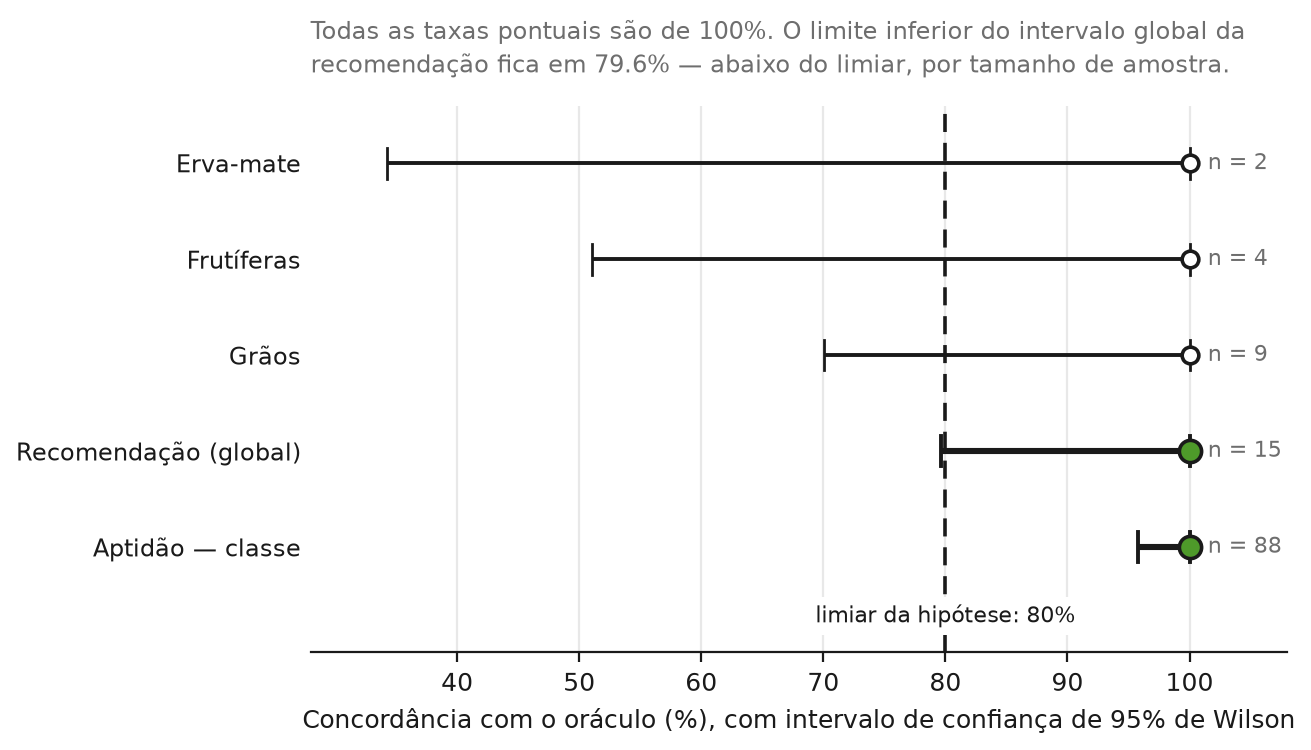
\includegraphics[width=0.95\textwidth]{fig/f7-concordancia}
\caption{Concordância com o oráculo, por grupo e global, com intervalo de confiança de 95\% de Wilson. Todas as taxas pontuais são de 100\%; o que o intervalo mostra é o efeito do tamanho da amostra, e o limite inferior do intervalo global da recomendação fica abaixo do limiar de 80\% que a hipótese estabelece.}
\label{fig:concordancia}
\end{figure}

Não houve caso discordante. Toda necessidade de calcário e toda dose de nitrogênio,
fósforo e potássio coincidiram com o valor calculado à mão, dentro da tolerância de
arredondamento declarada.

\textbf{O resultado precisa ser lido com a ressalva que ele próprio impõe.} Com 15 casos
e concordância integral, o limite inferior do intervalo de confiança de 95\% situa-se em
\textbf{79,6\%} --- isto é, \textbf{abaixo} do patamar de 80\% que a hipótese
H\textsubscript{1.1} estabelece. O resultado pontual satisfaz o critério; o intervalo,
por margem estreita, não. A causa não é erro do sistema, que acertou todos os casos, mas
o tamanho da amostra: com concordância integral, 16 casos elevariam o limite inferior a
80,6\% e 20 casos a 83,9\%.

\pendente{se mais casos forem calculados até a entrega, atualizar a tabela rodando
\texttt{python scripts/gera\_tabela\_concordancia.py} e reescrever este parágrafo com o
intervalo novo}

Duas observações sobre a natureza dessa evidência. A primeira é que o conjunto ficou
abaixo do alvo de 40 a 80 casos declarado no protocolo de validação, por restrição de
tempo: cada caso exige cálculo manual completo a partir do Manual, incluindo memória de
cálculo, e é esse custo que limita o conjunto. A segunda, e mais importante, é o
\textbf{risco de circularidade}: o sistema foi construído a partir do Manual e a
referência é o Manual aplicado pelo mesmo autor, de modo que o que se mede é a fidelidade
da implementação à transcrição --- não a adequação agronômica dos critérios. A mitigação
prevista é a incorporação de casos oriundos de laudos reais, com recomendação elaborada
por profissional habilitado, e o verificador do Anexo~1 citado na seção anterior é o
único oráculo hoje genuinamente externo.

\section{Conformidade do módulo de aptidão edáfica}

Para a aptidão, a verificação é de conformidade: mede se a implementação reproduz o
caderno de critérios aprovado, não se os critérios estão corretos. O conjunto tem 88
casos gabaritados, com o gabarito mantido em arquivo separado das entradas e gerado pela
aplicação manual da especificação, sem consulta ao código.

O resultado foi de \textbf{88/88 = 100\%} tanto na classe de aptidão atribuída quanto no
fator determinante, com intervalo de confiança de 95\% de [95,8\%; 100,0\%]. Conferir
também o fator determinante, e não apenas a classe, é o que impede que um acerto de
classe pelo motivo errado passe despercebido.

A ordem cronológica sustenta a alegação de não circularidade: a especificação foi
redigida e aprovada \textbf{antes} da implementação do motor, e o gabarito foi derivado
dela, não do código. Ao longo do desenvolvimento foram registradas oito divergências de
conformidade, todas analisadas individualmente e documentadas. Vale o registro de que
\textbf{nenhuma delas exigiu alterar um critério}: quatro eram lacunas de transcrição da
base, uma era erro de geração do gabarito, duas eram inconsistências de derivação entre
módulos --- resolvidas fazendo os dois derivarem da mesma grandeza, sem mudar limiar ---
e uma era defeito de arredondamento prematuro.

Convém, porém, não apresentar os dois "100\%" como se pesassem igual. A conformidade da
aptidão apoia-se em 88 casos e verifica a implementação contra uma especificação própria;
a concordância das recomendações apoia-se em 15 casos e verifica contra o Manual. A
segunda é a afirmação mais forte e a de evidência mais estreita.

\section{Comparação com ferramenta existente}

\pendente{executar a comparação com o FertFacil sobre um subconjunto dos casos e
escrever esta seção: convergências, divergências e sua explicação (diferença de critério
ou de edição do Manual), e as funcionalidades que o SIRAS oferece e a ferramenta
comparada não --- em especial a aptidão edáfica integrada e a trilha de inferência}

\section{Avaliação de usabilidade}

\pendente{seção inteira --- depende da coleta prevista para 20/10 a 14/11/2026. Rodar
\texttt{python scripts/consolidar\_heuristicas.py} sobre o CSV exportado do formulário e
escrever a partir da saída dele}

A seção deverá apresentar, nesta ordem: o perfil da amostra, a partir das perguntas de
caracterização do formulário; a conclusão das tarefas em cada roteiro; a tabela de
severidade por heurística, com média, mediana, mínimo e máximo; a lista de problemas
priorizada pela severidade; e a síntese das respostas abertas.

\pendente{perfil da amostra}
\pendente{conclusão das tarefas por roteiro}
\pendente{figura de severidade por heurística --- rodar
\texttt{scripts/consolidar\_heuristicas.py} sobre o CSV do formulário e depois
\texttt{scripts/gerar\_figuras\_artigo.py}, que só então produz
\texttt{fig/f8-usabilidade.png}. Inserir aqui com \texttt{label=fig:usabilidade}}
\pendente{lista priorizada de problemas, e quais foram corrigidos antes da entrega}
\pendente{síntese das quatro perguntas abertas, separando o juízo sobre a ferramenta do
juízo sobre a recomendação agronômica}

Na discussão desta seção, declarar as ameaças à validade já identificadas: o pesquisador
é o autor do sistema, o que tende a suavizar a crítica --- mitigado por responder o
questionário fora da sessão e sem a presença dele; o primeiro roteiro treina o
participante, de modo que o que se mede é adoção assistida, e não descoberta autônoma; e
a escala de severidade, atribuída por usuários a heurísticas em vez de por avaliadores a
problemas, exprime percepção de gravidade e não gravidade técnica.

\section{Discussão}

Os resultados disponíveis sustentam que a automatização dos critérios do Manual é
viável e que a implementação os reproduz com fidelidade: concordância integral nos casos
com oráculo, conformidade integral na aptidão e nenhuma falha não tratada em 367 estados
exercitados.

O diferencial declarado na introdução --- integrar recomendação de manejo e estimativa de
aptidão a partir de uma análise individual --- materializou-se na emissão conjunta dos
dois cenários de aptidão, atual e projetado, em que a diferença entre eles quantifica o
ganho atribuível à recomendação emitida. Nenhuma das ferramentas levantadas no
\cref{chap:revisao} produz essa saída.

Um resultado colateral merece registro por ilustrar o que a combinação de método
normativo e catálogo de mercado permite. Para a recomendação usada como exemplo pelo
próprio Manual, o sistema reproduz as três fórmulas que ele indica, com as doses
publicadas, e encontra ainda uma quarta --- de mesma proporção e igualmente exata ---
que consta de levantamento de fórmulas efetivamente utilizadas por produtores do Sul.
O método, sozinho, não a apontaria; o catálogo, sozinho, não saberia qual escolher.

As limitações mais relevantes são três, e nenhuma é contornável por esforço de
implementação. A primeira é a \textbf{circularidade parcial} da validação, já discutida.
A segunda é que a estimativa de aptidão é \textbf{exclusivamente edáfica}, sem relevo,
clima, drenagem ou suscetibilidade à erosão --- o que o próprio Manual indica como
necessário a uma avaliação de aptidão agrícola. A terceira é que a indicação de adubo
formulado faz um ranking \textbf{nutricional}, e não de custo: o Manual recomenda
escolher pelo menor custo por unidade de NPK, e o sistema não dispõe de preços, que são
do comprador e variam por revenda e por semana.

\pendente{fechar a discussão depois das seções 4.4 e 4.5, retomando o que a comparação
com a ferramenta existente e o teste com usuários acrescentaram}
